\documentclass[runningheads]{llncs}

%%%%%%%%%%%%%%%%%%%%%%%%
% Imports
%%%%%%%%%%%%%%%%%%%%%%%%
% \usepackage{minted} % Package for syntax highlighting (https://ctan.org/pkg/minted)
\usepackage[T1]{fontenc} % Standard package for selecting font encodings (https://ctan.org/pkg/fontenc)
\usepackage{color}
\usepackage{hyperref} % Extensive support for hypertext in LATEX (https://ctan.org/pkg/hyperref)
\usepackage{graphicx} % Enhanced support for graphics (https://ctan.org/pkg/graphicx). Should include EPS figures.
\usepackage{cite}
\usepackage{subfig}
\usepackage{geometry} % Change page size at any point
\usepackage[edges]{forest} % Drat tree like data structures (https://ctan.org/pkg/forest)
\usepackage{pgffor} % Loops in LaTeX (https://ctan.org/pkg/pgffor)
\usepackage{csvsimple} % Simple CSV file processing (https://ctan.org/pkg/csvsimple)
\usepackage{underscore} % Control the behaviour of "_" in text (https://ctan.org/pkg/underscore)
\usepackage{listings} % Typeset source code listings using LATEX (https://ctan.org/pkg/listings)
\usepackage[title]{appendix}
\usepackage{adjustbox}
\usepackage{tikz}
\usepackage{xspace}
\usepackage{wrapfig}
\usepackage{amsmath}
\usepackage{mathtools}
\usepackage{tikz}
\usepackage{algorithm}
\usepackage{algpseudocode}

%%%%%%%%%%%%%%%%%%%%%%%%
% Settings
%%%%%%%%%%%%%%%%%%%%%%%%
% \addto\extrasenglish{%
%     \providecommand*{\lstlistingautorefname}{List.}
%     % \renewcommand*{\listingscaption}{Code}
%     \renewcommand*{\equationautorefname}{Eq.}
%     \renewcommand*{\figureautorefname}{Fig.}
%     \renewcommand*{\chapterautorefname}{Chap.}
%     \renewcommand*{\sectionautorefname}{Sec.}
%     \renewcommand*{\subsectionautorefname}{Sub-sez.}
% }
\renewcommand\UrlFont{\color{blue}\rmfamily} % Change URL font
\urlstyle{rm} % Change URL style
\usetikzlibrary{arrows.meta} % Tikz library for arrows
\renewcommand{\algorithmicrequire}{\textbf{Input:}}
\renewcommand{\algorithmicensure}{\textbf{Output:}}

%%%%%%%%%%%%%%%%%%%%%%%%
% References
%%%%%%%%%%%%%%%%%%%%%%%%
% \addbibresource{resources.bib} %Import the bibliography file

%%%%%%%%%%%%%%%%%%%%%%%%
% Glossary
%%%%%%%%%%%%%%%%%%%%%%%%
% \makeglossaries
% \loadglsentries{glossary}

%%%%%%%%%%%%%%%%%%%%%%%%
% Minted
%%%%%%%%%%%%%%%%%%%%%%%%
% \setminted[solidity]{tabsize=2,breaklines,fontsize=\footnotesize}
% \setminted[typescript]{tabsize=2,breaklines,fontsize=\footnotesize}


%%%%%%%%%%%%%%%%%%%%%%%%
% Geometry
%%%%%%%%%%%%%%%%%%%%%%%%
\newcommand{\framedtext}[1]{%
    \par%
    \noindent\fbox{%
        \parbox{\dimexpr\linewidth-2\fboxsep-2\fboxrule}{#1}%
    }%
}

%%%%%%%%%%%%%%%%%%%%%%%%
% Listings
%%%%%%%%%%%%%%%%%%%%%%%%
\definecolor{keywords}{HTML}{C586C0}
\definecolor{type}{HTML}{0000FF}
\definecolor{operator}{HTML}{569CD6}
\definecolor{comments}{HTML}{6a9955}
\definecolor{variable}{HTML}{9e9b00}
\definecolor{number}{HTML}{098658}
\definecolor{function}{HTML}{795E26}

\lstset{language=C++,
    basicstyle=\ttfamily\small,
    keywordstyle=\color{keywords}\ttfamily,
    stringstyle=\color{orange}\ttfamily,
    commentstyle=\color{comments}\ttfamily,
    morecomment=[l][\color{comments}]{\#}
}
\lstdefinelanguage{SMT2}{
    alsoletter=-, % Include dashes as letters
    sensitive=true,
    morekeywords={set-logic, declare-fun, assert, check-sat, get-model},
    morekeywords=[2]{Int, Bool, Real},
    morekeywords=[3]{and, or, not, imply, ite},
    morekeywords=[4]{a, b, c, d, e, f, g, h, i, j, k, l, m, n, o, p, q, r, s, t, u, v, w, x, y, z},
    morecomment=[l]{;},
    morestring=[b]",
}
\lstset{
    language=SMT2,
    basicstyle=\ttfamily\small,
    keywordstyle=\color{keywords},
    keywordstyle={[2]\color{type}},
    keywordstyle={[3]\color{operator}},
    keywordstyle={[4]\color{variable}},
    commentstyle=\color{comments},
    stringstyle=\color{orange},
    showstringspaces=false,
    tabsize=2,
    breaklines=true,
}
\lstdefinelanguage{mps}{
    alsoletter=-, % Include dashes as letters
    sensitive=true,
    morekeywords={NAME, ROWS, COLUMNS, RHS, RANGES, BOUNDS, BINARIES, GENERALS, ENDATA},
    morekeywords=[2]{N, L, E, G, UP, LO, FX, FR, MI, PL},
    morecomment=[l]{*},
    morestring=[b]",
}
\lstset{
    language=mps,
    basicstyle=\ttfamily\small,
    keywordstyle=\color{keywords},
    keywordstyle={[2]\color{type}},
    commentstyle=\color{comments},
    stringstyle=\color{orange},
    showstringspaces=false,
    tabsize=2,
    breaklines=true,
}
\lstdefinelanguage{bazel}{
    alsoletter=-, % Include dashes as letters
    sensitive=true,
    morekeywords={load, workspace, http_archive, cc_binary, cc_library, cc_test, cc_toolchain, cc_toolchain_suite, filegroup, genrule, package_group, package, sh_binary, sh_library, sh_test},
    morekeywords=[2]{glob},
    morecomment=[l]{\#},
    morestring=[b]",
}
\lstset{
    language=bazel,
    basicstyle=\ttfamily\small,
    keywordstyle=\color{keywords},
    keywordstyle={[2]\color{function}},
    commentstyle=\color{comments},
    stringstyle=\color{orange},
    showstringspaces=false,
    tabsize=2,
    breaklines=true,
}
\lstdefinelanguage{yacc}{
    alsoletter={\#, \%, -, _, :}, % Include dashes as letters
    morekeywords={\#include, \#define, \#ifdef, \#endif},
    morekeywords=[2]{% Bison keywords
            \%union, \%token, \%type, \%nonassoc, \%left, \%prec, \%right, \%start,
            \%grammar, \%pure_parser, \%define, \%expect, \%expect-rr, \%file, \%glr-parser,
            \%parse-param, \%parse-param-rr, \%skeleton, \%debug, \%output,
            \%locations, \%skeleton
        },
    morekeywords=[3]{% Bison variables
            , stringVal,
        }
    keywordstyle=\color{keywords}\bfseries,
    morecomment=[l][\color{comments}]{//}, % single-line comments
    morecomment=[s][\color{comments}]{/*}{*/}, % multi-line comments
    morestring=[b]",
    morestring=[b]',
}
\lstset{
    language=yacc,
    basicstyle=\ttfamily\small,
    keywordstyle=\color{keywords},
    keywordstyle={[2]\color{type}},
    keywordstyle={[3]\color{variable}},
    commentstyle=\color{comments},
    stringstyle=\color{orange},
    showstringspaces=false,
    tabsize=2,
    breaklines=true,
}
\lstdefinelanguage{flex}{
    alsoletter={\#, \%, -, _, :}, % Include dashes as letters
    morekeywords={\#include, \#define, \#ifdef, \#endif},
    morekeywords=[2]{% Bison keywords
            typedef
        },
    morekeywords=[3]{% Bison variables
            , stringVal,
        }
    keywordstyle=\color{keywords}\bfseries,
    morecomment=[l][\color{comments}]{//}, % single-line comments
    morecomment=[s][\color{comments}]{/***}{*/}, % multi-line comments
    morestring=[b]",
    morestring=[b]',
}
\lstset{
    language=flex,
    basicstyle=\ttfamily\small,
    keywordstyle=\color{keywords},
    keywordstyle={[2]\color{type}},
    keywordstyle={[3]\color{variable}},
    commentstyle=\color{comments},
    stringstyle=\color{orange},
    showstringspaces=false,
    tabsize=2,
    breaklines=true,
}

%%%%%%%%%%%%%%%%%%%%%%%%
% Remove chapter header
%%%%%%%%%%%%%%%%%%%%%%%%
% \titleformat{\chapter}[display]{\normalfont\bfseries}{}{0pt}{\Huge}
% \newpagestyle{mystyle}
% {\sethead[\thepage][][\chaptertitle]{}{}{\thepage}}
% \pagestyle{mystyle}
% \AddToHook{env/appendices/begin}{%
%     \titleformat{\chapter}{\normalfont\LARGE\bfseries}{Appendix \thechapter}{10pt}{}%
% }

%%%%%%%%%%%%%%%%%%%%%%%%
% PlantUML
%%%%%%%%%%%%%%%%%%%%%%%%
\newcommand{\plantuml}[4][1]{
    \begin{figure}[h]
        \begin{adjustbox}{width=#1\textwidth,center}
            \input{#2}
        \end{adjustbox}
        \caption{#3}\label{dg:#4}
    \end{figure}
}

\newcommand{\wrapplantuml}[5][1]{
    \begin{wrapfigure}{#2}{#1\textwidth} %this figure will be at the right
        \centering
        \begin{adjustbox}{width=#1\textwidth,center}
            \input{#3}
        \end{adjustbox}
        \caption{#4}\label{dg:#5}
    \end{wrapfigure}
}

%%%%%%%%%%%%%%%%%%%%%%%%
% Equation caption
%%%%%%%%%%%%%%%%%%%%%%%%
\newcounter{eqcounter}
\newcommand{\eqcaption}[1]{
    {
            \medskip
            \centering
            \setcounter{eqcounter}{\theequation}
            Equation \theeqcounter: #1
            \addtocounter{eqcounter}{1}

            \vskip-0.5\baselineskip
            \noindent
        }
}

%%%%%%%%%%%%%%%%%%%%%%%%
% Common definitions
%%%%%%%%%%%%%%%%%%%%%%%%
\def\dlinear{\textit{dLinear}\xspace}
\def\pydlinear{\textit{pydLinear}\xspace}
\def\dlinearfive{\textit{dLinear5}\xspace}
\def\dlinearfour{\textit{dLinear4}\xspace}
\def\bazel{\textit{Bazel}\xspace}
\def\dreal{\textit{dReal4}\xspace}
\def\soplex{\textit{SoPlex}\xspace}


%%%%%%%%%%%%%%%%%%%%%%%%%%
% ---- Begin document ----
%%%%%%%%%%%%%%%%%%%%%%%%%%
\begin{document}

% ---- Metadata ----
\title{\dlinear: an SMT QF\_LRA Solver Supporting Floating Point Arithmetic and Delta-Completeness}
\titlerunning{\dlinear}

\author{Ernesto Casablanca\inst{1}
    %\orcidID{0009-0009-3741-1624}
    \and
    Martin Jonathan O'Connor Sidaway\inst{1}
    %\orcidID{0000-0001-6481-1169}
    \and
    Sadegh Soudjani\inst{2}
    %\orcidID{0000-0003-1922-6678}
    \and
    Paolo Zuliani\inst{3}
    %\orcidID{0000-0001-6481-1169}
}
\authorrunning{E. Casablanca et al.}

\institute{Newcastle University, Newcastle upon Tyne, United Kindgom\\
    \email{\{e.casablanca2,?martin?\}@newcastle.ac.uk} \and % TODO: add martin's email and ensure orcidID
    Max Planck Institute for Software Systems, Kaiserslautern, Germany\\
    \email{sadegh@mpi-sws.org} \and
    La Sapienza University, Rome, Italy\\
    \email{zuliani@di.uniroma1.it}}

%%%%%%%%%%%%%%%%%%%%%
% ---- Sections ----
%%%%%%%%%%%%%%%%%%%%%

% ---- Title page ----
\maketitle

% ---- Abstract ----
\begin{abstract}
    \dlinear is an SMT solver for the theory of linear real arithmetic (QF\_LRA).
    It uses floating point arithmetic to verify the feasibility of the linear constraints instead of the traditional fully rational approach utilised by other state of the art SMT solvers,
    while still guaranteeing an exact solution.
    Furthermore it allows for delta-complete reasoning, which relaxes the constraints by an arbitrary factor to produce the output faster.

    \keywords{SMT \and Delta-complete \and Floating point arithmetic}
\end{abstract}

% ---- Introduction ----
\section{Introduction}

A propositional formula is a construct that uses \textit{variables} (or \textit{unknowns}), which are assigned a semantic value \textbf{True} or \textbf{False}, and \textit{logical connectives}, such as $\lor$ (or), $\land$ (and) and $\neg$ (not).
A literal is a variable $x$ or its negation $\neg x$.
Propositional formulae are usually expressed in the Conjunctive normal form (CNF), which is to say as a conjunction of clauses, where a clause is a disjunction of literals (see Eq.~\ref{eq:cnf-notations}).
A generic propositional formula can be converted into and equisatisfiable CNF formulation through the Tseitin encoding~\cite{ref:handbook-sat}.
If a clause contains exactly one literal, it is called a unit clause.
Lastly, an empty clause, that is, a clause with no literals, corresponds to the formula $\bot$.
\begin{equation}
    \label{eq:cnf-notations}
    \begin{gathered}
        \bigwedge_{i=1}^n \bigvee_{j=1}^{m_i} l_{ij} \\
        ( l_{00} \lor l_{01} \lor \dots \lor l_{0m_0}) \land (l_{10} \lor l_{11} \lor \dots \lor l_{1m_1}) \land \dots \land (l_{n0} \lor l_{n1} \lor \dots \lor l_{nm_n}) \\
        \{ \{ l_{00}, l_{01} , \dots , l_{0m_0} \} , \{ l_{10} , l_{11} , \dots , l_{1m_1} \}, \dots , \{ l_{n0} , l_{n1} , \dots , l_{nm_n} \} \}
    \end{gathered}
\end{equation}
\eqcaption{Three notations used to represent a CNF formula with $n$ clauses and $m_i$ literals in the $i$-th clause.}

A \textbf{SAT solver} is a procedure able to determine whether a given propositional formula is satisfiable, that is, if there exists a boolean assignment of values to the variables that makes the formula true.
Although the problem is generally \textbf{NP-complete}~\cite{ref:np-sat}, over the years many efficient algorithms have been developed to tackle it, with the most popular being the Conflict Driven Clause Learning (\textbf{CDCL}) algorithm~\cite{ref:handbook-sat}, which started as an extension of the original Davis–Putnam–Logemann–Loveland \textbf{DPLL} algorithm~\cite{ref:dpll} with additional key techniques, such as learning clauses and from conflicts and exploiting their structure~\cite{ref:conflict-driven-clause-learning}, lazy data structures and low efficient branching heuristics~\cite{ref:watched-literals}.
CDCL is employed in most recent state-of-the-art SAT solvers, such as the version of \textit{Minisat} in cvc5~\cite{ref:cvc5-smt-comp-2022} and \textit{Glucose}~\cite{ref:glucose}.

Satisfiability for propositional formulas can be extended to Satisfiability Modulo Theories (\textbf{SMT}).
Let $\Sigma$ be a signature containing predicate and function symbols, with their arity, where $\Sigma^F$ is the set of functions and $\Sigma^P$ the set of predicates.
Furthermore, let the 0-arity symbols of $\Sigma^F$ be constants, and the 0-arity symbols of $\Sigma^P$ propositions.
A ground ($\Sigma$-)term $t$ is defined as a constant, the application of a function symbol to a list of terms compatible with its arity.
A ground ($\Sigma$-)formula $\varphi$ can be a proposition, a predicate over a list of terms, an equality between terms, the symbols $\top$ or $\bot$ or any logical connectives $\land$, $\lor$, $\neg$, $\implies$ and $\iff$ applied to other $\Sigma$-formulas.
Lastly, the term $ite$, known as the if-then-else operator, is defined in terms of three elements: a formula and two terms.
\begin{equation}
    \label{eq:smt-notations}
    \begin{gathered}
        \begin{array}{lll}
            A \in \Sigma^P & \text{arity } 0   & \text{proposition} \\
            c \in \Sigma^F & \text{arity } 0   & \text{constant}    \\
            p \in \Sigma^P & \text{arity } > 0 & \text{predicate}   \\
            f \in \Sigma^F & \text{arity } > 0 & \text{function}    \\
        \end{array}
        \\
        \begin{array}{lrll}
            t       & \coloneqq & c                                                          & \text{ground term}    \\
                    & \mid      & f(t_1, \ldots, t_n)                                                                \\
                    & \mid      & ite(\varphi, t_1, t_2)                                                             \\
            \\
            \varphi & \coloneqq & A                                                          & \text{ground formula} \\
                    & \mid      & p(t_1, \ldots, t_n)                                                                \\
                    & \mid      & t_1 = t_2 \mid \top \mid \bot  \mid \neg\varphi                                    \\
                    & \mid      & \varphi_1 \land \varphi_2 \mid \varphi_1 \lor \varphi_2                            \\
                    & \mid      & \varphi_1 \implies \varphi_2 \mid \varphi_1 \iff \varphi_2                         \\
        \end{array}
    \end{gathered}
\end{equation}
\eqcaption{Notations used to represent a SMT formula}
Literals in SMT formulas represent an \textbf{atom}, that is to say a proposition, a predicate, an equality between terms or the symbols $\top$ or $\bot$.
Formulae can be assigned a semantic meaning, \{\textbf{true}, \textbf{false}\}, by applying a \textbf{model} $\mathcal{A}$, which is a pair consisting of a non empty set $A$ and a mapping from all constant symbol $c \in \Sigma^F$ to an element $a^\mathcal{A} \in A$, from each function symbol $f \in \Sigma^F$ of arity $n > 0$ to a total function $f^\mathcal{A} : A^n \to A$, from each proposition $B \in \Sigma^{P}$ to a boolean value $b \in \{\textbf{true}, \textbf{false}\}$ and finally from each predicate symbol $p \in \Sigma^P$ of arity $n > 0$ to a total function $p^\mathcal{A} : A^n \to \{ \textbf{true}, \textbf{false} \}$.
The mapping in the model determines the \textit{interpretation} of the formula.
Following the expected conversions, for any $\mathcal{A}$
\begin{gather*}
    f(t_1, \dots, t_n)^{\mathcal{A}} = f^{\mathcal{A}}(t_1^{\mathcal{A}}, \dots, t_n^{\mathcal{A}}) \\
    p(t_1, \dots, t_n)^{\mathcal{A}} = p^{\mathcal{A}}(t_1^{\mathcal{A}}, \dots, t_n^{\mathcal{A}}) \\
    ite(\varphi, t_1, t_2)^{\mathcal{A}} = \begin{cases}
        t_1^{\mathcal{A}} & \text{if } \varphi^{\mathcal{A}} = \textbf{true}  \\
        t_2^{\mathcal{A}} & \text{if } \varphi^{\mathcal{A}} = \textbf{false}
    \end{cases} \\
    \bot = \textbf{false} \quad \top = \textbf{true}
\end{gather*}
If follows that a model $\mathcal{A}$ \textbf{satisfies} a formula $\varphi$ if $\varphi^{\mathcal{A}} = \textbf{true}$.
To conclude with some definitions, we say that a set $\Gamma$ of ground formulae \textbf{entails} a ground formula $\varphi$, denoted $\Gamma \models \varphi$, iff every model $\mathcal{A}$ that satisfies all formulae in $\Gamma$ satisfies $\varphi$ as well.
$\Gamma$ is \textbf{consistent} iff $\Gamma \not\models \bot$ and it is \textbf{valid} iff $\emptyset \models \Gamma$.

While these definitions are extremely generic, it is common to restrict the signature $\Sigma$ to a specific theory $\mathcal{T}$, such as the theory of linear real arithmetic (\textbf{QF\_LRA}), the theory of bit-vectors (\textbf{QF\_BV}), the theory of arrays (\textbf{QF\_AUFLIA}) and many others~\footnote{SMT-LIB officially supported logics: \url{https://smt-lib.org/logics.shtml}}.
Then, the problem of satisfiability is the problem of determining whether if is exists an interpretation within the chosen theory that satisfies the formula $\varphi$.
The same problem can also be formulated as a validity problem, for to satisfy $\varphi$ means that $\neg\varphi$ must be valid and vice versa.

The tool presented in this paper will focus on the QF\_LRA theory.
The interpretation uses the domain $\bbbr$ of real numbers.
Furthermore, only $+, -, \times,$ arithmetic operators are allowed, with $\times$ being restricted to multiply a variable only by a constant.
Therefore, each atom can be expressed in the form $a_1x_1 + \ldots + a_nx_n \bowtie b$, where $x_i \in \bbbr \forall i \in \{1, 2, \dots, n\}$ are the variables, $a_i, b \in \bbbr \quad \forall i \in \{1, 2, \dots, n\}$ are the constants and $\bowtie \in \{<, \le, =, \ne, \ge, >\}$.
With these restriction in place, the QF\_LRA theory is decidable.
The area of application we are interested in is the verification of big Neural Networks (NNs) and other machine learning models.
The input space of these models is often very large, and the constraints that need to be verified are often piecewise linear.

It is easy to see how the QF\_LRA theory is very closely related to the Linear Programming (LP) problem.
A linear program is a mathematical optimisation problem where the objective function to maximise and the constraints the solution is subject to are linear.
LP problems are formulated in the \textit{standard form} (Eq.~\ref{eq:lp-standard}), where the objective function is to be maximised, the constraints are all $\le$ inequalities and the variables are non-negative.
The conversion to the standard form is always possible and can be done in polynomial time.
\begin{equation}
    \label{eq:lp-standard}
    \begin{split}
        \text{Maximise }   \quad & \sum_{i=1}^{n} c_i x_i                      \\
        \text{subject to } \quad & \sum_{i=1}^{n} a_{ji}x_{i} < b_j            \\
                                 & x_i \ge 0,  \quad i \in \{1, 2, \ldots, n\}
    \end{split}
\end{equation}
\eqcaption{Standard form of a Linear Programming problem with $n$ variables and $m$ constraints.}

The most commonly used algorithm to solve LP problems is the Simplex method~\cite{ref:simplex}.
While having a worst-case exponential time complexity, it is often very efficient in practice.
Unfortunately, most out-of-the-shelf implementations do not handle strict inequalities, which are common in SMT problems.
We will discuss how to handle them in Section~\ref{sec:lra-theory-solver}.

State-of-the-art SMT solvers such as Z3~\cite{ref:z3} and CVC5~\cite{ref:cvc5} already fully support the (QF\_LRA) theory.
Their approach uses a rational numerical representation applied to a specialised Simplex-based~\cite{ref:simplex} solver to guarantee an exact solution and support strict inequalities, usually ignored by LP solvers.
Unfortunately, rational arithmetic operations do not offer a constant time complexity. % TODO: find a better source or add empirical evidence
Unlike floating point arithmetic, the time required to complete the computation grows based on the size of the rational representation, which is not fixed, and the algorithm used~\cite{ref:fft-mult}, hence it can slow down the calculation significantly.
While in the LP community a tradeoff between precision and speed of the tool usually favors the former, with many commercial tools utilising floating point arithmetic~\cite{ref:gurobi}, this is not considered a viable option in the context of SMTs.
Inexact procedures would not guarantee completeness, as rounding errors are introduced in the computation.

Some alternative methods have been developed during the years.
The \textit{QSoptex} solver \footnote{QSoptex: \url{https://www.math.uwaterloo.ca/~bico/qsopt/ex/index.html}} uses a technique called \textbf{incremental precision boosting}~\cite{ref:precision-boosting}.
Working with floating-point numbers with variable precision, the algorithm increments the number of bits used in their representation until the solution is found and checking it using a rational number representation only to confirm its correctness.
A approach is to utilise an \textbf{iterative refinement algorithm}~\cite{ref:iterative-refinement} such as the one implemented in \soplex \footnote{SoPlex: \url{https://soplex.zib.de/}}.
This variation starts by solving the original problem with a fixed precision before considering a sequence of related LP instances that only differ in the variables' bounds, the constraints' sides and the objective function coefficients.
These subtasks translate in a shift/zoom of the original LP instance, increasing the initial output's precision.
The process is iterated until the desired resolution is reached.
Some subroutines are in place to check for unsoundness and infeasibility in the presence of approximations derived from the floating-point arithmetic.

% ---- Architecture ----
\section{Architecture}

\wrapplantuml[0.5]{r}{diagrams/dpll}{DPLL(T)-based SMT solver}{dpll}
\dlinear implements the standard DPLL(T)-based~\cite{ref:dpll-t} SMT solver structure utilised in most other state-of-the-art solvers~\cite{ref:z3-dpll-t}.
DPLL(T)-based solvers the lazy approach to SMT solving, being comprised of two main components interacting with each other (see Figure~\ref{dg:dpll}).
A boolean \textbf{SAT solver} which aims to satisfy the initial formula by assigning a $true$ or $false$ value to each theory-literal, and a \textbf{theory solver} which checks the consistency of the literals that have been assigned a value.
If no conflicts are found, a model is returned, terminating the process.
Otherwise, it is the theory solver's responsibility to generate an explanation, which takes the form of one or more learned clauses to add to the formula, to force the SAT solver to backtrack and try a different assignment.
If the SAT solver is unable to find a satisfying assignment, the formula is declared unsatisfiable.

More formally, given an input boolean formula, usually in CNF, the SAT solver is prompted to produce an assignment
\begin{equation} % Taken from Martin's thesis
    \label{eq:smt-formula}
    \varphi = t_1(x) \le 0 \wedge \ldots \wedge t_m (x) \le 0
\end{equation}
where
\begin{equation*}
    t_i(x) = A_{i1}x_1 + \ldots + A_{in}x_n - b_i, \quad 1 \le i \le m
\end{equation*}
and $x \in \bbbr^n, A \in \bbbr^{m \times n}, b \in \bbbr^m$, satisfying $\varphi$ means verifying that
\begin{equation*}
    \exists x \in \bbbr^n : t_1(x) \le 0 \wedge \ldots \wedge t_m(x) \le 0
\end{equation*}
which is a formulation for a LP problem without an objective function.

In the case of \dlinear, the theory solver converts the linear constraints of the assigned literals into constraints of an LP problem fed to the LP solver.
\dlinear offers the option to utilise a elementary theory preprocessor able to cheaply detect simple unsatisfiable linear constraints and produce a conflict clause without the need to call the LP solver.
Furthermore, \dlinear is able to parse MPS files, a standard format for LP problems, by implicitly creating a single assertion the LP solver will try to satisfy.

% ---- Linear Real Arithmetic theory ----
\section{Linear Real Arithmetic theory solver}
\label{sec:lra-theory-solver}

\subsection*{Preprocessing}

\dlinear implements some of the common preprocessing strategies when it comes to optimising the performance solver for the QF\_LRA theory.
All simple equality bounds are propagated using the problem's constraints in a graph-like structure (Figure~\ref{dg:preprocessor}).
If one or more conflicts are detected, the original atoms are traced back and used to generate the explanations.
This also allows to further guide the theory solver, by adding additional bounds to the variables, which further reduce the search space.
The preprocessing can still be disabled by the user if its contribution is negligible, if not detrimental, to the overall performance on the given instance.

\begin{figure}[h]
    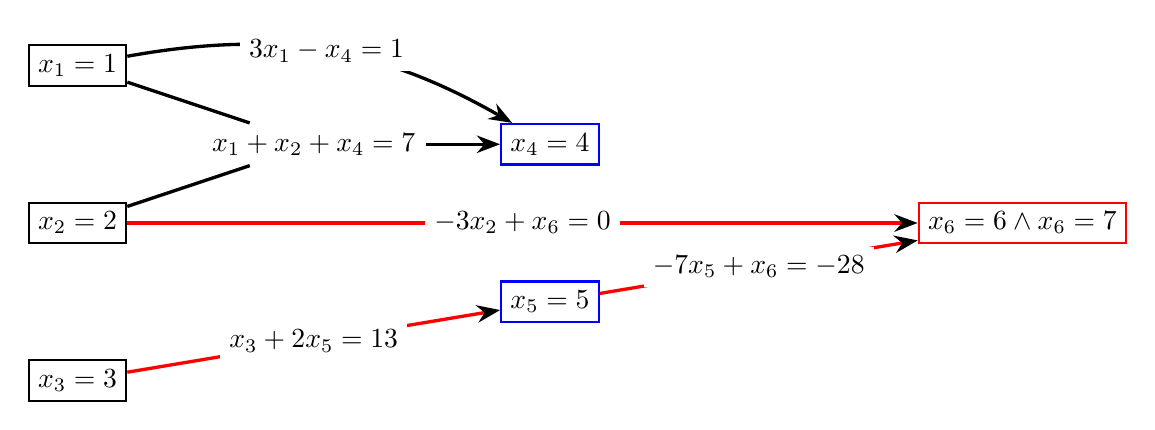
\begin{tikzpicture}
        \begin{scope}[every node/.style={rectangle,thick,draw}]
            \node (1) at (0,4) {$x_1 = 1$};
            \node[shape=rectangle,draw=none] (a) at (3,3) {$x_1 + x_2 + x_4 = 7$};
            \node (2) at (0,2) {$x_2 = 2$};
            \node (3) at (0,0) {$x_3 = 3$};
            \node[shape=rectangle,draw=blue] (4) at (6,3) {$x_4 = 4$};
            \node[shape=rectangle,draw=blue] (5) at (6,1) {$x_5 = 5$};
            \node[draw=red] (6) at (12,2) {$x_6 = 6 \land x_6 = 7$};
        \end{scope}

        \begin{scope}[>={Stealth[black]},
            every node/.style={fill=white,rectangle},
            every edge/.style={draw=black,very thick}]
            \path [-] (1) edge (a);
            \path [-] (2) edge (a);
            \path [->] (a) edge (4);
            \path [->] (1) edge[bend left=20] node {$3x_1 -  x_4 = 1$} (4);
            \path [->] (3) edge[draw=red] node {$x_3 + 2x_5 = 13$} (5);
            \path [->] (2) edge[draw=red] node {$-3x_2 + x_6 = 0$} (6);
            \path [->] (5) edge[draw=red] node {$-7x_5 + x_6 = -28$} (6);
        \end{scope}
    \end{tikzpicture}
    \caption{Example of a preprocessor graph. The given bounds (the nodes on the left) propagate using the constraints, inducing additional bounds (the blue nodes) that can be used to guide the solver.
        If a conflict is detected (red node), the edges responsible (red edges) are traced back to the origin to formulate an explanation to add to the SAT solver.
        In this case, the explanation adds the clause $(\neg l_1 \lor \neg l_2 \lor \neg l_3 \lor \neg l_4 \lor \neg l_5)$ where $l_1 \coloneqq x_2 = 2, l_2 \coloneqq x_3 = 3, l_3 \coloneqq -3x_2 + x_6 = 0, l_4 \coloneqq x_3 + 2x_5 = 13, l_5 \coloneqq -7x_5 + x_6 = -28$.
        Graphically, at least one of the red edges or the nodes from which they originate must be absent.}
         \label{dg:preprocessor}
\end{figure}

\subsection{LP solver}

The LP solver used by \dlinear by default is \soplex.
It implements both the incremental precision boosting and the iterative refinement algorithms.
The user can choose between the two, or even an hybrid approach.
The LP solver is used to verify the feasibility of the constraints.
Because we are not interested in the optimal solution but in finding any solution, a low hanging fruit in terms of optimisation is to set the objective function to $0$ to avoid pointless computations.
This is not the case in our implementations as we will see in section~\ref{sec:strict-bounds}.

If a feasible solution is found, it means that the original formula is satisfiable, and the assignment is returned to the user.
Note that there is no guarantee of uniqueness of the solution, so adding an artificial clause with the negation of the solution found will lead to another solution being found or the formula being declared unsatisfiable.
On the other hand, if the LP problem is infeasible, we can use the Farkas Ray to determine the irreducible inconsistent subsystem of the original problem, and use it to produce an explanation.

\subsection{Strict bounds}
\label{sec:strict-bounds}

To use out-of-the-box LP solvers as theory solvers, some adjustments in the formulation of the input may be required.
A common optimisation technique is to drop the objective function, setting it to $0$.
Strict inequalities are common place in SMT formulas, but they are usually not supported by LP solvers, for they would make the feasible region no longer closed, possibly making the search for the optimal solution pointless.
Other state-of-the-art SMT solver employing rational arithmetic withing the theory solver~\footnote{z3 documentation: \url{https://z3prover.github.io/papers/z3internals.html\#sec-rational-linear-arithmetic}}, use a symbolic variable representing an infinitesimal parameter $\delta$ witch enforces the inequality~\cite{ref:lra-dpll-t}.
Since our goal is to verify feasibility, we can reformulate the problem into an equi-feasible one, while getting rid of the strict inequalities at the cost of losing the original objective function.
To do so, introduce a new variable called \textbf{strict variable}, $t$.
To simplify the notation, we only consider $<$ strict inequalities, but the same reasoning can be applied to $>$, since they can always be converted to $<$ by multiplying both sides by $-1$.
Following the standard LP notation, let us indicate with $x_1, x_2, \ldots, x_n \in \bbbr$ the \textbf{decision variables}, $a_{11}, a_{12}, \ldots, a_{mn}, b_{2}, \ldots, b_{m}\in \bbbr$ some constants, with $J$ the set of indexes of strict inequality constraints and with $K$ the set of indexes for all other constraints.
Start by replacing each strict inequality
\begin{align*}
    \sum_{i=1}^{n} a_{ji}x_{i} < b_j, \quad \forall j \in J
\end{align*}
with equivalent non strict inequalities using the strict variable $t$:
\begin{align*}
    \sum_{i=1}^{n} a_{ji}x_{i} + t \le b_j, \quad \forall j \in J \\
    t > 0
\end{align*}
This change would only move the strict inequality problem to the bound on $t$.
However, it is possible to go a step further and relax the newly introduced bound by changing the objective function to maximise $t$.
The original problem we want to verify the feasibility of
\begin{equation}
    \label{eq:lp-original}
    \begin{split}
        \text{Maximise }   \quad & 0                                                          \\
        \text{subject to } \quad & \sum_{i=1}^{n} a_{ji}x_{i} < b_j,   \quad \forall j \in J  \\
        \quad                    & \sum_{i=1}^{n} a_{ki}x_{i} \le b_k,  \quad \forall k \in K \\
                                 & x_i \ge 0,  \quad i \in \{1, 2, \ldots, n\},
    \end{split}
\end{equation}
can be relaxed to
\begin{equation}
    \label{eq:lp-relaxed}
    \begin{split}
        \text{Maximise }   \quad & t                                                             \\
        \text{subject to } \quad & \sum_{i=1}^{n} a_{ji}x_{i} + t \le b_j, \quad \forall j \in J \\
        \quad                    & \sum_{i=1}^{n} a_{ki}x_{i} \le b_k, \quad \forall k \in K     \\
                                 & x_i \ge 0 , \quad i \in \{1, 2, \ldots, n\}                   \\
                                 & t \ge 0
    \end{split}
\end{equation}

\begin{theorem}
    \label{thm:lp-relaxed}
    The original problem \eqref{eq:lp-original} is feasible if and only if the relaxed problem \eqref{eq:lp-relaxed} is feasible and there exists a solution where the objective value is greater than $0$.
\end{theorem}

A bigger challenge is represented by \textit{not equal to} ($\ne$) constraints.
Two strict inequalities are needed to check whether the constraint is satisfied, one for each direction.
Since checking both at the same time with an OR conjunction is not possible, the original problem must be split into two.
If the number of not equal constraints is $m$, then $2^m$ problems must be solved.
If any of them is feasible, then it is possible to conclude that the original problem is feasible.
Some smarter heuristics can improve the average performance of the solver.
For instance, there is no need to continue solving subproblems if none of the \textit{not equal to} constraints appear in the explanation for last infeasibility, and if only exactly one of them appears, we can discard all other subproblems where it appears with with the same sense.

% ---- Delta-completeness ----
\section{delta-completeness}

\dlinear offer the option to use delta-completeness.

% Taken from Martin's thesis
\begin{definition}
    If $\varphi$ is a Boolean formula in which every atomic formula is of one the forms $t = 0$ or $t \le 0$ where $t$ is an arbitrary term, then the $\delta$-weakening of $\varphi$, denoted $\varphi^{-\delta}$, is, for any $\delta > 0$, the formula obtained by replacing every atomic formula $t = 0$ with $|t| \le \delta$, and every atomic formula $t \le 0$ with $t \le \delta$ (or, equivalently, $t - \delta \le 0$).
\end{definition}
If $\varphi$ is defined as in (Eq.~\ref{eq:smt-formula}), then $\varphi^{-\delta}$ can be written as
\begin{equation*}
    \varphi^{-\delta} = t_1(x) \le \delta \land \ldots \land t_m(x) \le \delta
\end{equation*}
and its satisfiability problem can be written in linear algebra notation as
\begin{equation}
    \label{eq:delta-sat}
    \exists x \in \bbbr^n : |Ax - b| \le \delta 1^m
\end{equation}
where $1^\sigma = [1, \ldots, 1]$ denotes a vector of ones of size $\sigma$.
\begin{definition}
    A $\delta$-complete decision procedure for satisfiability over a class of formulas $F$ is an algorithm that, if provided as input any formula $\varphi \in F$, terminates and outputs (non-deterministically) exactly one of the following symbols:
    \begin{enumerate}
        \item unsat only if $\varphi$ is unsatisfiable
        \item $\delta$-sat only if $\varphi^{-\delta}$ (the $\delta$-weakening of $\varphi$) is satisfiable
    \end{enumerate}
\end{definition}
Note that this is non-deterministic, because both conditions can simultaneously be true.
Furthermore, any complete method is, by definition, trivially $\delta$-complete.
The advantage of this approach is given by the fact that the LP solver can stop refining the solution as soon as the arbitrary precision $\delta$, indicated by the user, is reached, possibly saving computation time, especially for numerically challenging instances.

% ---- Benchmarks ----
\section{Benchmarks}

\subsection*{Specifications}

We compared \dlinear with the following state-of-the-art tools: cvc5~\cite{ref:cvc5} (version 1.0.8), Z3~\cite{ref:z3} (version 4.12.2).
The benchmarking suite has been run on a machine running CentOs with 2 Intel Xeon E5-2699 v4 processors @ 2.2 GHz, 22 cores, 55 MB cache with a memory limit of 2.9GB (DDR4 RDIMMs).
The timeout was set to 6 hours.

\subsection*{Result}


\begin{credits}
    \subsubsection{\ackname} This study was funded by EPSRC
\end{credits}

% ---- Bibliography ----
\bibliographystyle{splncs04}
\bibliography{resources}

% ---- Appendices ----
% \begin{appendices}
%     Proof of~\autoref{thm:lp-relaxed}.
%     \chapter{Proof}
%     \begin{proof}
%         Without loss of generality, assume that both linear programming problems are in standard form.
%         Let $J$ be the set of indexes of strict inequality constraints, and $K$ be the set of indexes for all other constraints.
%         \\
%         \framedtext{\eqref{eq:lp-original} feasible $\implies$ \eqref{eq:lp-relaxed} feasible $\land$  \eqref{eq:lp-relaxed} objective value $> 0$} \\

%         If the original problem is feasible, then there exists a solution, a set of values to be assigned to the decision variables $x_1, x_2, \ldots, x_n$, that satisfies all the constraints.
%         For the strict inequality constraints to be satisfied, it means that there exists a value $\delta_j > 0, \quad j \in J$ such that
%         \begin{align*}
%             \sum_{i=1}^{n} a_{ji}x_{i} + \delta_j = b_j, \quad \forall j \in J
%         \end{align*}
%         Let $\bar{t} = \min(\delta_j), \quad j \in J$.
%         The expression becomes
%         \begin{align*}
%             \sum_{i=1}^{n} a_{ji}x_{i} + \bar{t} \le b_j, \quad \forall j \in J \\
%             \bar{t} > 0
%         \end{align*}
%         which is the formulation of the previously strict constraints used in the relaxed problem.
%         All other constraints have been left unchanged, therefore the solution to the original problem can be used to satisfy the constraints of the relaxed problem by also setting $t = \bar{t}$ which is greater than $0$.
%         Hence, the objective value of the relaxed problem is $> 0$.
%         \\
%         \framedtext{\eqref{eq:lp-relaxed} feasible $\land$  \eqref{eq:lp-relaxed} objective value $> 0$ $\implies$ \eqref{eq:lp-original} feasible} \\

%         The solution to the relaxed problem already satisfies all the non-strict constraints of the original problem.
%         The objective value is greater than $0$; therefore, $t > 0$.
%         Since all relaxed constraints in the form
%         \begin{align*}
%             \sum_{i=1}^{n} a_{ji}x_{i} + t \le b_j, \quad \forall j \in J \\
%             t > 0
%         \end{align*}
%         are satisfied the original strict inequality constraints
%         \begin{align*}
%             \sum_{i=1}^{n} a_{ji}x_{i} < b_j, \quad \forall j \in J
%         \end{align*}
%         are also satisfied.
%         Hence, the original problem is feasible.
%     \end{proof}

% \end{appendices}

\end{document}
